\apendice{Documentación de usuario}

\section{Introducción}
En este anexo mostramos en que sistemas se puede usar la aplicación y bajo qué condiciones de manera que la puedan usar los clientes.

\section{Requisitos de usuarios}
El único requisito que necesita un usuario que quiera usar nuestro sistema es un navegador. Necesitamos \eng{javascript} y \eng{cookies} activados, las \eng{cookies} son para mantener la sesión.

Navegadores con los que se ha comprobado:
\begin{enumerate}
\item Firefox 53 
\item Chrome 57
\end{enumerate}


\section{Instalación}
Al proporcionar nuestro servicio como una página web no necesitamos que el cliente o usuario instale la aplicación. 

Si de todas las maneras se hubiese decidido que cada usuario tiene la aplicación en su ordenador, se pueden seguir las instrucciones del manual de instalación para usuarios avanzados [\ref{sec:ins}].

\section{Manual del usuario}
El manual de usuario es más simple que otras aplicaciones, esto se debe a que el enfoque del proyecto no ha sido tanto tener una aplicación con muchas funcionalidades, sino seguir un proceso de desarrollo que permitiera utilizar algunas de las tecnologías de desarrollo más en boga actualmente. He querido aprovechar la realización del proyecto como una oportunidad de formación y aprendizaje adicional al realizado en el grado, y de este modo mejorar mi preparación de cara a la inserción en el mercado laboral.
\FloatBarrier
El usuario generalmente llegará a la aplicación por su índice o portada. A esta página generalmente se accede con la dirección IP 127.0.0.1 si la ejecución es local.

\begin{figure}
	\centering
	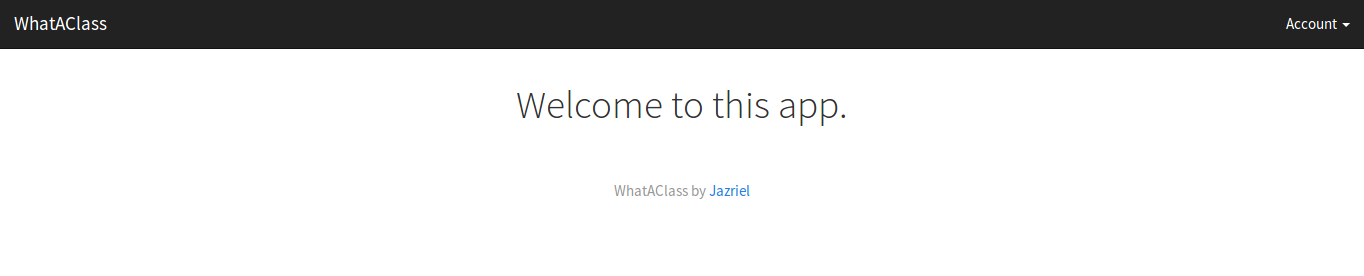
\includegraphics[width=1\textwidth]{index.png}
	\caption{Punto de entrada a la aplicación}\label{fig:index.png}
\end{figure}

Para usar la aplicación a partir de ese punto necesita registrarse o iniciar sesión con una de las opciones de inicio de sesión alternativas.
\begin{figure}
	\centering
	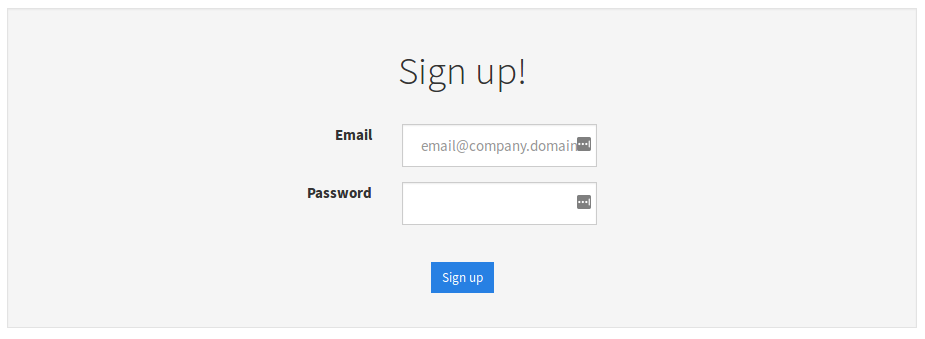
\includegraphics[width=1\textwidth]{signup.png}
	\caption{Pantalla de registro de usuario}\label{fig:signup.png}
\end{figure}

Tras registrarse como usuario o tripulante, si esta preparado el correo, se envía un correo electrónico a su dirección personal.
\begin{figure}
	\centering
	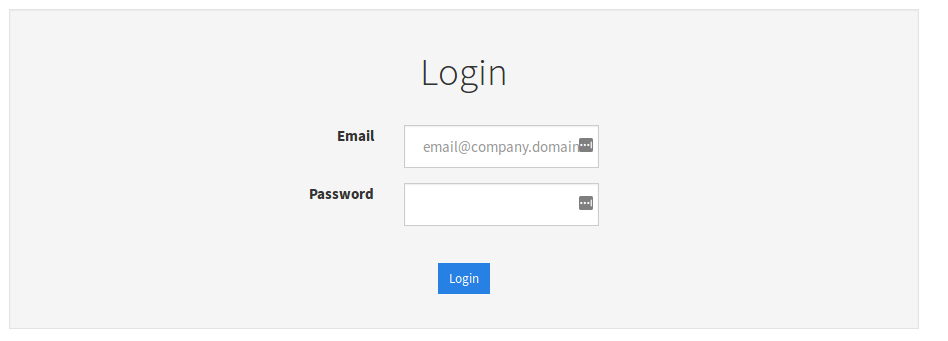
\includegraphics[width=1\textwidth]{login.png}
	\caption{Pantalla de inicio de sesión}\label{fig:login.png}
\end{figure}

\begin{figure}
	\centering
	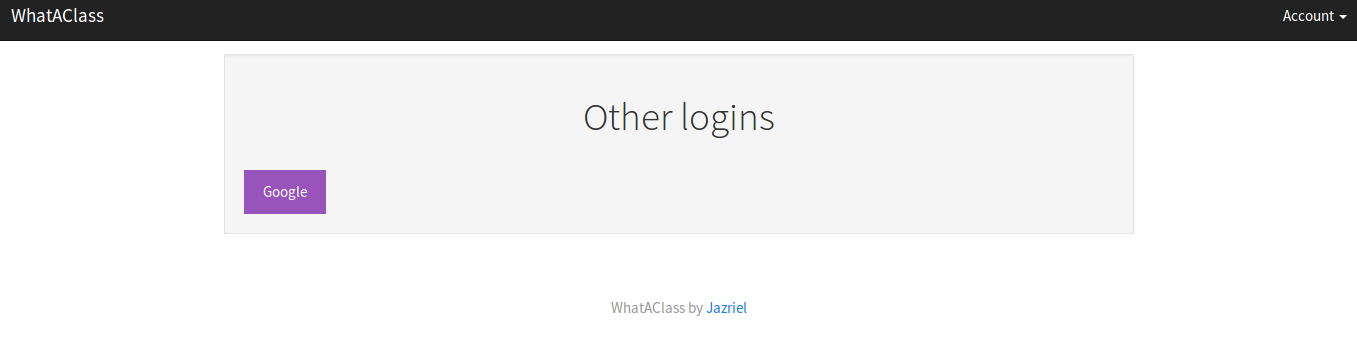
\includegraphics[width=1\textwidth]{other_logins.png}
	\caption{Inicios de sesión alternativos}\label{fig:other_logins.png}
\end{figure}

\FloatBarrier
Una vez se confirma la recepción del correo, se activa la cuenta, permitiendo así usar servicios que antes no estaban disponibles.

\begin{figure}
	\centering
	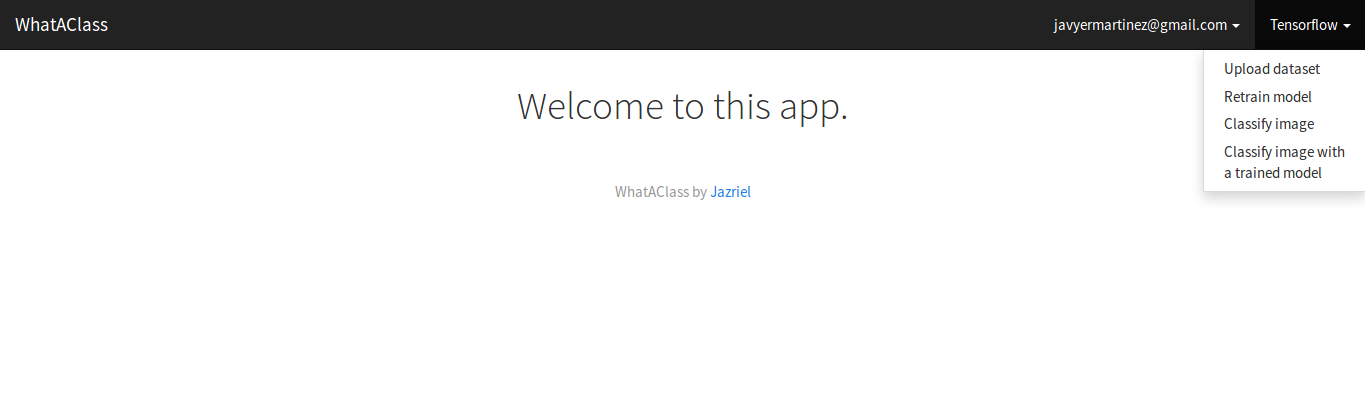
\includegraphics[width=1\textwidth]{loggedin.png}
	\caption{Cambio de las zonas accesibles al iniciar sesión}\label{fig:loggedin.png}
\end{figure}


\begin{figure}
	\centering
	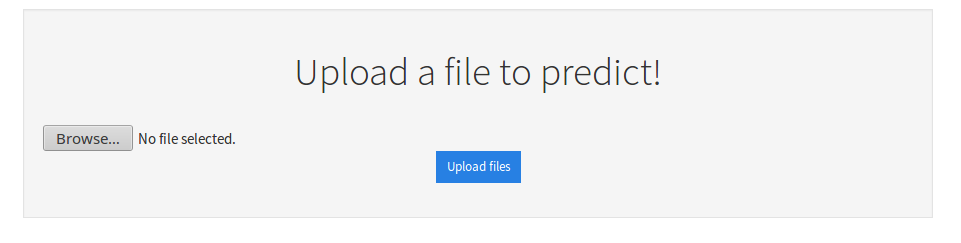
\includegraphics[width=1\textwidth]{predict.png}
	\caption{Pantalla de acceso al servicio de clasificación}\label{fig:predict.png}
\end{figure}

\begin{figure}
	\centering
	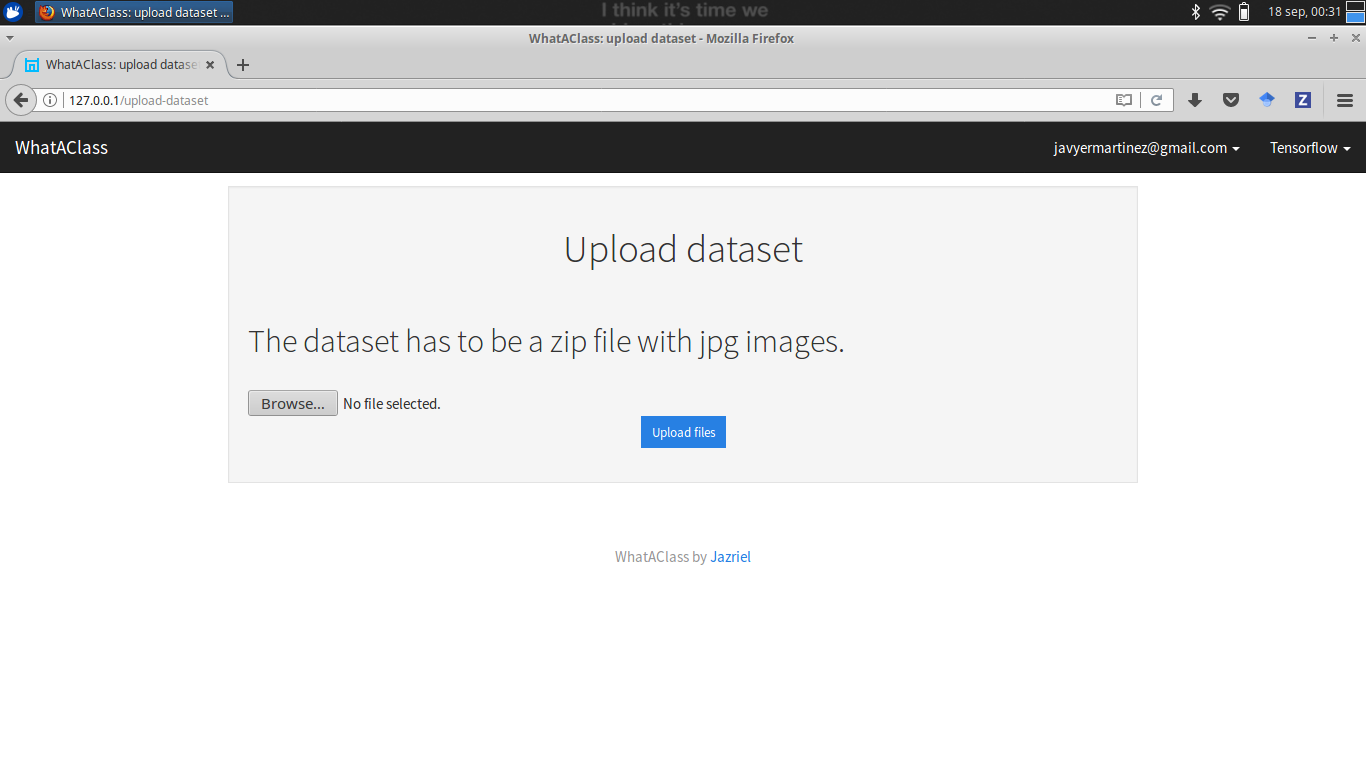
\includegraphics[width=1\textwidth]{up_dataset.png}
	\caption{Pantalla de subida del dataset}\label{fig:up_dataset.png}
\end{figure}


\begin{figure}
	\centering
	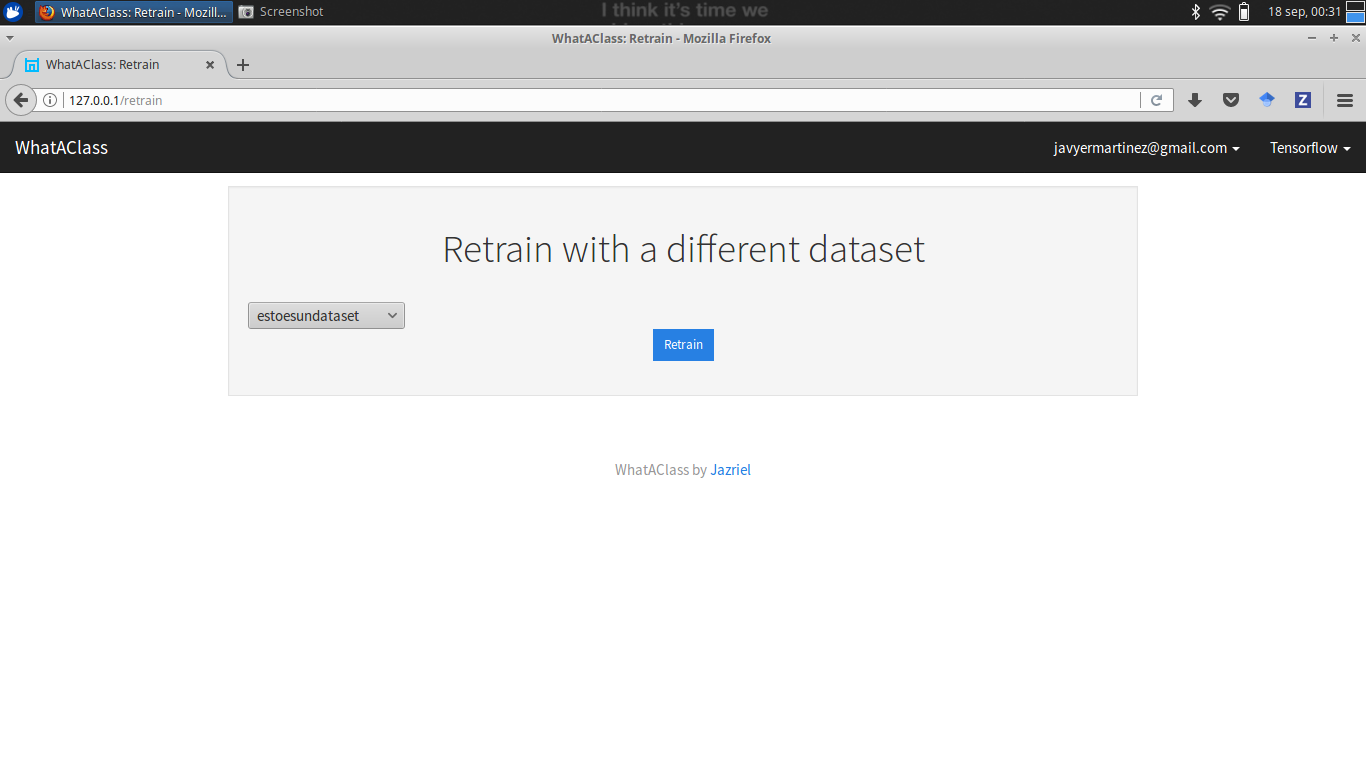
\includegraphics[width=1\textwidth]{retrain.png}
	\caption{Pantalla de reentrenamiento del modelo}\label{fig:retrain.png}
\end{figure}


\begin{figure}
	\centering
	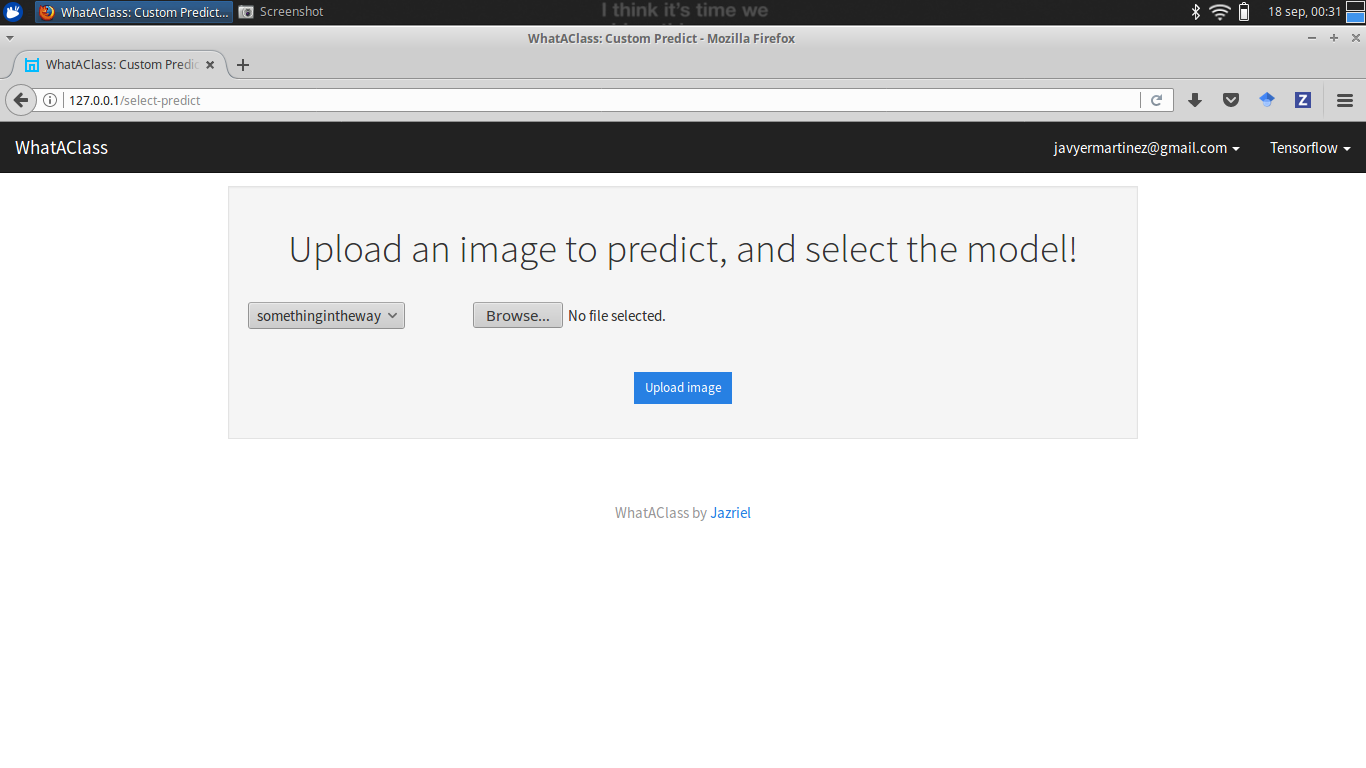
\includegraphics[width=1\textwidth]{select_predict.png}
	\caption{Pantalla del servicio de clasificación tras el reentrenado}\label{fig:select_predict.png}
\end{figure}

\begin{figure}
	\centering
	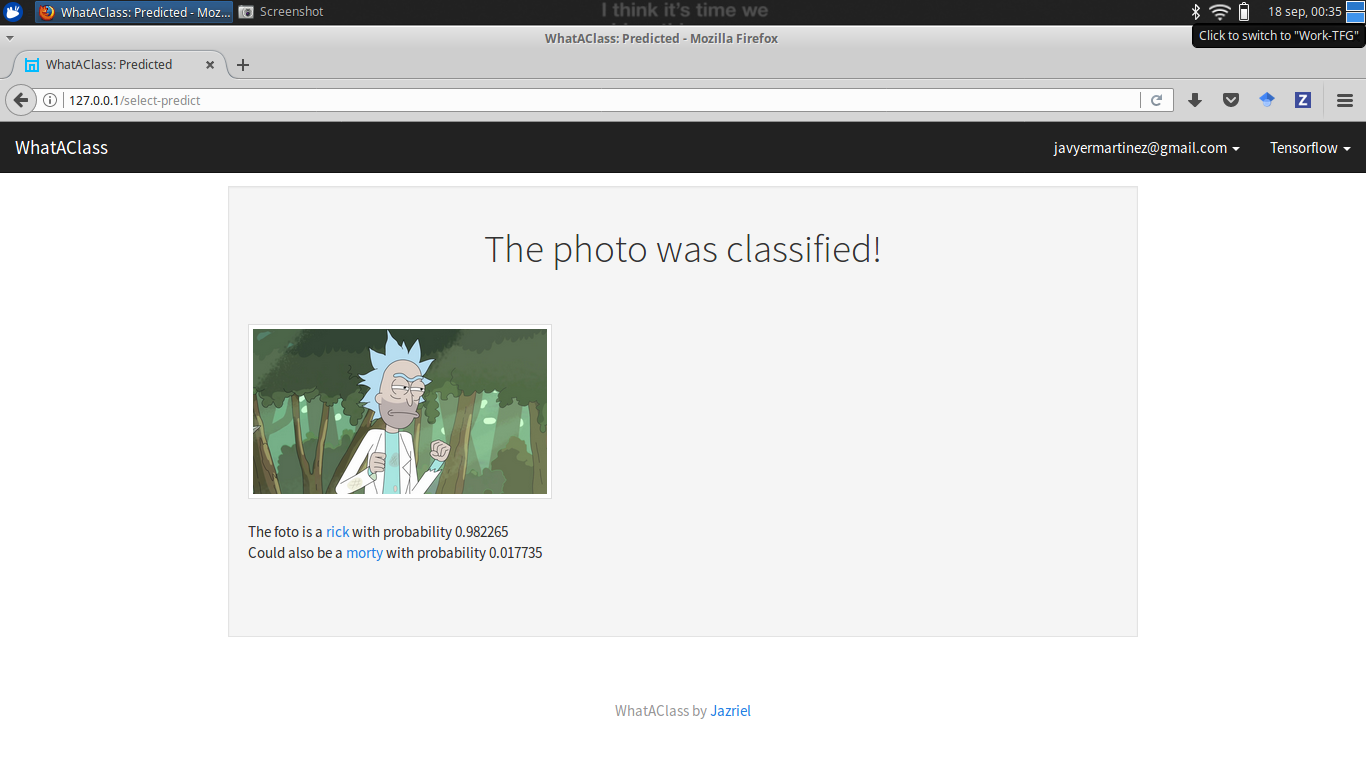
\includegraphics[width=1\textwidth]{custom_class.png}
	\caption{Pantalla de clasificación tras reentrenado del modelo}\label{fig:custom_class.png}
\end{figure}








